\chapter{Revisão Bibliográfica} \label{chap:sota}

%\section*{}

%\section{Introdução}

\section{Workflow}
Um \textit{workflow} consiste num conjunto de tarefas com dependências lógicas ou de dados que podem ser executadas por diferentes nós num sistema computacional. Para obter uma execução eficiente de um conjunto de \textit{workflows} é necessária uma técnica de escalonamento que minimize o \textit{Turnaround Time}.

Um típico workflow científico pode ser representado por um grafo acíclico direcionado (DAG). Num DAG, nós representam tarefas e arestas direcionadas representam dependências de execução e a quantidade de comunicação entre nós. Um \textit{workflow} é modelado através de um DAG $G = (V,E)$, onde $V = {nj, j = 1..v}$ representa o conjunto de v tarefas a executar e E representa o conjunto de arestas direcionadas e representa requisitos de comunicação entre tarefas \cite{Arabnejad}.

Num dado DAG, uma tarefa sem predecessores é denominada tarefa de entrada e uma tarefa sem sucessores é denominada tarefa de saída.
Assumimos que um DAG tem exatamente uma tarefa de entrada e uma tarefa de saída. Se um DAG tem múltiplas tarefas de entrada ou de saída, uma tarefa de entrada ou saída falsa com peso 0 e 0 arestas é adicionada ao grafo \cite{ArabnejadUP}

\begin{figure}[H]
	\centering
	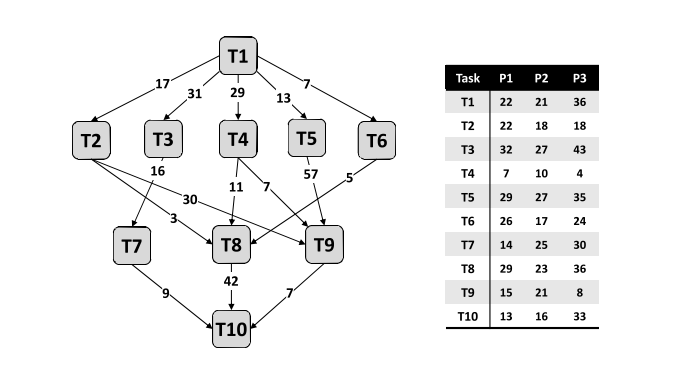
\includegraphics[width=0.6\textwidth]{exemploWorkflow.png}
	\caption{Exemplo de um workflow}
	\label{workflow}
\end{figure}


Um exemplo de um DAG pode ser visto na Figura \ref{workflow}, que representa um DAG e um sistema de computação com 3 processadores e os correspondentes custos de comunicação e computação. Na figura \ref{workflow}, o peso de cada aresta representa o seu custo de comunicação médio e os número na tabela o tempo de computação em cada um dos 3 processadores. \cite{Arabnejad}. 


\section{Métricas de Desempenho}
Para quantificar a performance de uma técnica de escalonamento de \textit{workflows} existem uma série de métricas que têm sido aplicadas pelos investigadores desta área. Nesta secção é explicado o seu significado.

\subsection{Makespan}
\textit{Makespan} ou \textit{Schedule Length} é o tempo entre o início da execução do nó de entrada de um \textit{workflow} e o final da execução do nó de saída desse mesmo \textit{workflow}.
É definido por: $makespan = AFT(nsaída)-AST(nentrada)$ onde AFT(nsaída) simboliza o \textit{Actual Finish Time} (tempo actual de finalizaçao) do nó de saída e AST(nentrada) simboliza o \textit{Actual Start Time} (tempo actual de começo) do nó de entrada.
\cite{Arabnejad}

Também por vezes denominado \textit{Schedule Length}
A maior parte dos algoritmos de escalonamento utilizam esta métrica para mostrar e avaliar os seus resultados e soluções em comparação com outros algoritmos.
Um menor \textit{makespan} implica uma melhor performance.
\cite{Arabnejad}

\subsection{Turnaround Time}
O \textit{Turnaround Time} é a diferença de tempo entre a submissão de um \textit{workflow} e a conclusão do processamento do mesmo. É diferente do \textit{makespan}na medida
em que inclui o tempo que o \textit{workflow} fica em espera. É utilizado para medir a performance e satisfação na perspectiva do utilizador.\cite{Arabnejad}
Esta métrica vai ser importante neste trabalho, visto ser direcionada a medir a satisfação do utilizador, o nosso parâmetro mais importante para medir QoS.

\subsection{Turnaround Ratio}
O \textit{Turnaround Ratio} mede o tempo adicional que cada \textit{workflow} gasta no sistema à espera de ser executado em relação ao \textit{makespan} desse \textit{workflow}.\cite{Arabnejad}

\section{Clusters}
Um \textit{cluster} é um tipo de sistema paralelo ou distribuído que consiste num conjunto de computadores independentes interconectados (nós), que trabalham em conjunto como um único recurso computacional integrado. Um nó computacional pode ser um sistema com um ou mais processadores (PCs, \textit{workstations}, servidores, etc.), com memória, processadores gráficos e um sistema operativo \cite{Buyya1999}.
\textit{Cluster} geralmente refere-se a 2 ou mais computadores (nós) ligados entre si. Os nós podem existir numa única prateleira ou podem estar fisicamente separados e conectados por uma LAN.
A figura \ref{cluster} ilustra uma típica arquitetura de um cluster.

\begin{figure}[H]
	\centering
	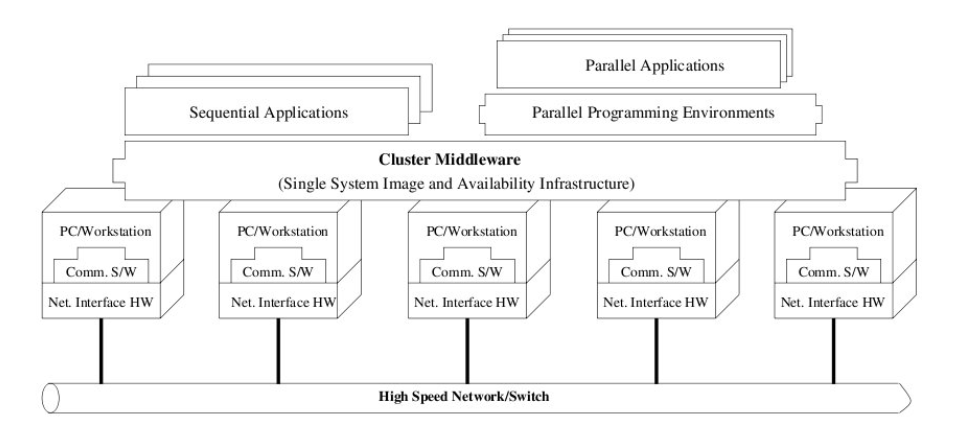
\includegraphics[width=0.6\textwidth]{cluster.png}
	\caption{Arquitetura de um Cluster}
	\label{cluster}
\end{figure}

Os algoritmos de escalonamento de workflows concorrentes são úteis quando o número de workflows excede o número de processadores nos vários nós de um cluster. Caso contrário, os workflows poderiam usar um conjunto de processadores exclusivamente sem concorrência. 
No caso da MEO, o cluster consiste em três servidores conectados na mesma rede.
Numa rede comutada, a execução de tarefas e comunicação podem ser conseguidas em cada processador simultaneamente e sem contenção. Este facto ajuda a simplificar a computação dos custos de comunicação nos DAGs, considerando apenas os parâmetros de comunicação médios \cite{Arabnejad}.

\section{Técnicas de Escalonamento para workflows concorrentes}
Uma operação de escalonamento consistem em definir um mapeamento e ordem para execução de tarefas\cite{Arabnejad}

Recentemente, vários algoritmos têm sido propostos para escalonamento de \textit{workflows} concorrentes com o objetivo de melhorar o tempo de execução de várias aplicações em sistemas computacionais. A maior parte destes algoritmos foram desenvolvidos para escalonamento off-line, ou seja, em que todas as aplicações são conhecidas ao mesmo tempo. Esta abordagem, apesar de relevante, impõe limitações na gestão de um sistema dinâmico em que utilizadores podem submeter trabalhos a qualquer altura. Para este propósito, existem alguns algoritmos que foram concebidos para lidar com escalonamento em aplicações dinâmicas.\cite{Arabnejad}. 

Para um dedo cenário que inclua um conjunto de \textit{workflows} submetidos em diferentes alturas por vários utilizadores, o objetivo é encontrar um mapeamento de tempo que garanta cumprir certas restrições de QoS, como por exemplo, o \textit{Turnaround Time} do pré-processamento de um vídeo não pode demorar mais do que 2 vezes o tempo de processamento sem concorrência (\textit{deadline}).
O tempo de conclusão (ou \textit{Turnaround Time}), como referido anteriormente, inclui tanto o tempo de espera como o tempo de execução de um \textit{workflow}, estendendo a definição de \textit{makespan}. \cite{Kwok1999}

\subsection{Escalonamento Off-line}
O escalonamento off-line caracteriza-se por ter os \textit{workflows} disponíveis antes do início da execução. 
Quando um escalonamento é produzido e aplicado, mais nenhum \textit{workflow} é considerado. 
Esta abordagem, apesar de limitada, aplica-se em muitos casos reais, como por exemplo, quando um utilizador tem um conjunto de nós para correr um conjunto de \textit{workflows}. 
Esta metodologia costuma ser aplicada pelas ferramentas de gestão de recursos mais comuns quando um utilizador reserva um conjunto de nós para executar os seus trabalhos exclusivamente. 

Vários algoritmos foram propostos para escalonamento off-line nos quais \textit{workflows} competem por recusos. O objectivo é garantir uma distribuição justa desses recursos e minimizar o \textit{Turnaround Time} de cada \textit{workflow}. 

Zhao e Sakellariou \cite{Zhao2006} apresentaram duas abordagens baseadas numa estratégia justa de escalonamento de \textit{workflows} concorrentes. 
A justiça é definida na base do atraso (rácio entre o tempo de execução esperado para um DAG quando escalonado com outro(s) \textit{workflows} e sozinho) que cada \textit{workflow} experienciaria.
Propuseram dois algoritmos, um com uma política de justiça baseada no tempo de término e um com uma política de justiça baseada no tempo atual.
Inicialmente, ambos os algoritmos mapeiam cada DAG para todos os processadores utilizando uma técnica de escalonamento estático (como HEFT \cite{Topcuoglu2002} ou Hybrid.BMCT \cite{Sakellariou2004}) como algoritmo de escalonamento de articulação.
Posteriormente, guardam o mapeamento atribuído e o seu \textit{makespan} como o valor de atraso do DAG. Depois, todos os \textit{workflows} são ordenados em ordem decrescente de atraso. Finalmente, enquanto houverem \textit{workflows} por processar na lista, o algoritmo seleciona o DAG com o maior atraso e  a primeira tarefa disponível que ainda não foi agendada neste DAG.
A ideia do algoritmo é avaliar o valor do atraso de cada DAG depois de escalonar uma tarefa e decidir qual deverá ser o próximo DAG a ser selecionado para escalonar a próxima tarefa.
A diferença entre os dois algoritmos propostos é que o com a política de equidade baseado no tempo de término apenas calcula o atraso do DAG selecionado, enquanto que o com a política de equidade baseada no tempo atual o valor do atraso é recalculado para cada DAG.

N’takpé e Suter \cite{NTakpe2009} propuseram várias estratégias baseadas na partilha proporcional de recursos. Esta partilha proporcional foi definida com base no comprimento do caminho crítico, largura ou esforço associado a cada DAG. Foi também proposta uma partilha proporcional ponderada que representa um melhor equilíbrio entre partilha justa de recursos e a redução do \textit{makespan} dos \textit{workflows}. As estratégias foram propostas e aplicadas a aplicações paralelas mistas, onde cada tarefa pode ser executada em mais que um processador. A partilha proporcional baseada no esforço necessário para executar um \textit{workflow} obteve os resultados menos demorados em média, mas por outro lado foi também menos justa no que toca à utilização de recursos, ou seja, a variação entre os atrasos experienciados foi a mais alta.

Bittencourt e Madeira \cite{Bittencourt2010} propuseram uma heurística de \textit{clustering} de caminhos que combina a técnica de escalonamento de clustering para gerar grupos (\textit{clusters}) de tarefas e uma tecnica de lista de escalonamento para selecionar tarefas e processadores. Com base nesta metodologia, Bittencourt e Madeira propõem e comparam quatro algoritmos, que são:
\begin{itemize}
	\item escalonamento sequencial, onde \textit{workflows} são agendados um a seguir ao outro
	\item algoritmo de procura de abertas, que é semelhante ao anterior mas procura abertas entre tarefas já agendadas
	\item algoritmo de intercalação, onde partes de cada workflow são agendadas por turnos
	\item \textit{workflows} de grupo, onde os \textit{workflows} são agregados para formar um único workflow e depois escalonados como tal.
\end{itemize} 
A avaliação foi feita em termos do comprimento do agendamento e justiça e concluiu-se que intercalar os workflows leva a um menor \textit{makespan} em média e maior equidade quando múltiplos workflows partilham o mesmo conjunto de recursos. Os resultados, apesar de relevantes, consideram o \textit{makespan} médio, que não distingue o impacto do atraso em cada \textit{workflow} quando comparado com uma execução exclusiva.

Casanova et al. \cite{Casanova2010} avaliaram extensivamente algoritmos de escalonamento off-line de tarefas concorrentes paralelas num único \textit{cluster} homogéneo.
Os DAGs ou workflows submetidos por utilizadores diferentes partilham um conjunto de recursos e estão prontos a iniciar a sua execução ao mesmo tempo. O objetivo é optimizar a percepção do utilizador de desempenho e justiça. Os autores propuseram 3 métricas para quantificar a qualidade de um escalonamento relacionadas com desempenho e equidade entre os diferentes DAGs de tarefas paralelos.

Carbajal et al. \cite{Hirales-Carbajal2012} apresentaram 2 algoritmos de escalonamento de \textit{workflows}:
\begin{itemize}
	\item MWGS4	- Multiple Workflow Grid Scheduling 4 stages
	\item MWGS2 - Multiple Workflow Grid Scheduling 2 stages
\end{itemize} 
Estes algoritmos consistem em 4 e 2 fases: \textit{labeling}, alocação adaptativa, priorização e escalonamento de máquinas paralelas. Ambos os algoritmos estão classificados como estratégias off-line e mapeiam um conjunto de trabalhos disponíveis e prontos a ser executados pertencentes a um lote de trabalhos. Todos os trabalho que chegarem num intervalo de tempo serão processados num lote e começarão a ser executados quando o processamento de lote de trabalho anterior estiver concluído. Foi mostrado que as estratégias propostas superam outras estratégias em termos de tempo de espera médio do caminho crítico e atraso do caminho crítico.

\subsection{On-line Scheduling}
O escalonamento on-line é caracterizado por ter um comportamento dinâmico onde \textit{workflows} podem ser submetidos por utilizadores a qualquer altura.
Quando se faz um escalonamento de vários \textit{workflows} independentes que representam trabalhos de utilizadores e são submetidos em instantes diferentes no tempo, o \textit{Turnaround Time} toma em conta quer o tempo de espera quer o tempo de execução de um dado \textit{workflow}, estendendo a definição de \textit{makespan} para escalonamento de um único \textit{workflow} \cite{Kwok1999}. A métrica para avaliar um escalonador dinâmico de \textit{workflows} independentes tem que representar o tempo individual de conclusão em vez de uma medida global para o conjunto de \textit{workflows}, de modo a medir a QoS experienciada pelos utilizadores, estando esta relacionada com o tempo de conclusão de cada submissão de um utilizador.

Alguns algoritmos foram propostos para escalonamento de \textit{workflows} on-line. Três outros foram propostos especificamente para escalonar workflows concorrentes com o objetivo de melhorar o QoS individual de cada \textit{workflow}. Estes algoritmos, On- line Workflow Management (OWM), Rank Hybrid (Rank Hybd) e Fairness Dynamic Workflow Scheduling (FDWS), são detalhados e comparados na próxima secção.

Liu et al. \cite{Liu2009} propuseram o algoritmo MMA(Min-Min Average) para escalonar eficientemente \textit{workflows} com muitas transações que envolvem \textit{overheads} de comunicação consideráveis em grelhas computacionais. 
O algoritmo MMA é baseado no algoritmo Min-Min, mas usa uma estratégia diferente, que lhe permite adaptar-se às variações de velocidade da rede que liga a grelha automaticamente. \textit{Workflows} com muitas transações são muitas instâncias de um \textit{workflow} e o objetivo do MMA é otimizar a taxa de transferência, ao invés da performance individual de cada \textit{workflow}. 

Xu et al. \cite{Xu2009} propuseram um algoritmo para escalonamento de múltiplos \textit{workflows} com múltiplas restrições ed QoS para a \textit{Cloud}. O algoritmo \textit{Multiple QoS Constrained Scheduling Strategy of Multiple Workflows} (MQMW) minimiza o \textit{makespan} e o custo dos recursos e aumenta a taxa de sucesso de escalonamento. O algoritmo considera dois objetivos, tempo e custo, que podem ser adaptados às necessidades dos utilizadores. Este algoritmo foi comparado ao \textit{Rank Hybd} e quando tempo era o principal requisito de QoS, o \textit{Rank Hybd} obteve melhor desempenho. Visto que o tempo é o nosso principal requisito de QoS, este algoritmo não vai ser testado. 

Barbosa e Belmiro \cite{Barbosa2011} propuseram um algoritmo dinâmico para minimizar o \textit{makespan} de um lote de \textit{workflows} paralelos com tempos de chegada diferentes. O algoritmo foi proposto para escalonamento on-line mas com o objetivo de minimizar uma métrica global. Este modelo é aplicado em cenários reais como videovigilância, registo de imagens e outros, nos quais os \textit{workflows} estão relacionados e como tal apenas o resultado colectivo é significativo. Esta abordagem é diferente da que diz respeito a esta dissertação.


\section{Algoritmos de Escalonamento} \label{sec:schalg}

\subsection{Algoritmo Rank Hybrid}
Yu e Shi in \cite{Yu2008} propuseram uma estratégia \textit{planner-guided} strategy, de nome Rank Hybd, para lidar com o escalonamento dinâmico de \textit{workflows} submetidos por utilizadores distinto em intervalos de tempo diferentes.

\begin{figure}[H]
	\centering
	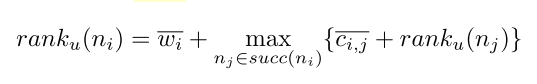
\includegraphics[width=0.6\textwidth]{ranku.png}
	\caption{Fórmula de $rank_u$}
	\label{ranku}
\end{figure}

O algoritmo \textit{Rank Hybd} atribui uma classificação a todas as tarefas utilizando a medida de prioridade $rank_u$ \cite{Topcuoglu2002}, que representa o tamanho do caminho mais longo de uma tarefa $n_i$ até ao nó de saída de um DAG, incluindo o custo computacional de $n_i$ e pode ser visto na Figura \ref{ranku}. Aqui, succ($n_i$) representa o conjunto de sucessores imediatos da tarefa $n_i$, $c_{i,j}$ é o custo médio de comunicação da aresta(i,j) e $w_i$ é o custo médio de computação da tarefa $n_i$. Para a tarefa de saída, $rank_u(n_{exit}) = 0$.

\begin{figure}[H]
	\centering
	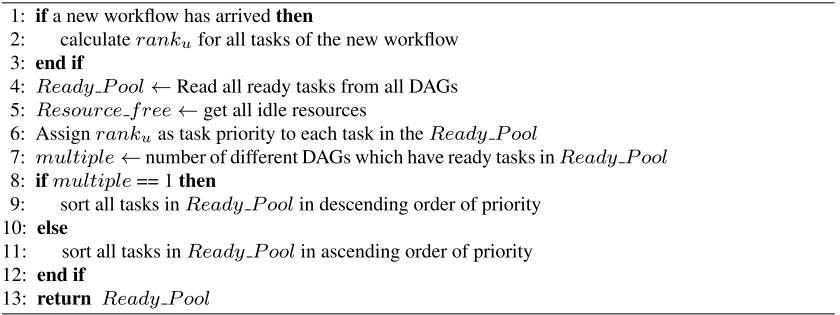
\includegraphics[width=0.6\textwidth]{rankHybdAlg1.png}
	\caption{Algoritmo 1 do Rank Hybd}
	\label{rankHybdAlg1}
\end{figure}


\begin{figure}[H]
	\centering
	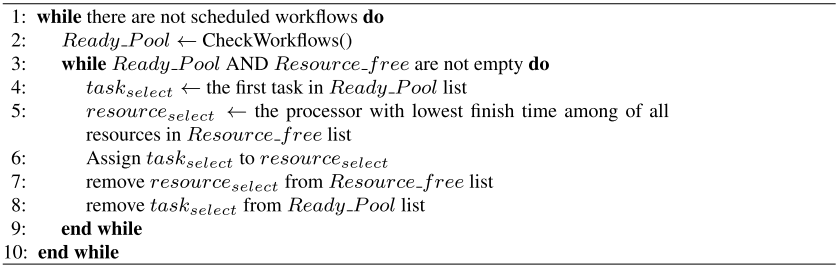
\includegraphics[width=0.6\textwidth]{rankHybdAlg2.png}
	\caption{Algoritmo 2 do Rank Hybd}
	\label{rankHybdAlg2}
\end{figure}

A cada passo, o algoritmo lê todas as tarefas disponíveis em todos os DAGs e seleciona a próxima tarefa a mapear de acordo com a sua classificação. Se as tarefas disponíveis pertencem a DAGs diferentes, o algoritmo seleciona a tarefa com a classificação mais baixa. Caso contrário, a tarefa com classificação mais alta é selecionada. A heurística do \textit{Rank Hybd} é formalizada na figura \ref{rankHybdAlg2} \cite{Arabnejad}.

Recorrendo a esta estratégia, o algoritmo \textit{Rank Hybd} permite que o DAG com classificação mais baixa (e \textit{makespan} mais baixo) seja mapeado primeiro para reduzir o tempo de espera do DAG no sistema. No entanto, esta estratégia não é particularmente justa para todos os \textit{workflows}. Isto porque dá sempre preferência a workflows mais pequenos e adia os \textit{workflows} maiores. Se um \textit{workflow} grande estiver a ser executado e forem submetidos vários \textit{workflows} mais pequenos, o escalonador adiará a execução do \textit{workflow} maior para dar prioridade aos mais pequenos.

\subsection{Algoritmo Online Workflow Management}
Hsu et al. \cite{Hsu2011} propuseram o algoritmo OnlineWork- flow Management (OWM) para escalonamento on-line de múltiplos workflows.
O algoritmo começa por selecionar uma tarefa disponível de cada DAG, a que tiver maior classificação ($rank_u$, Figura \ref{ranku}) e colocá-las na lista de tarefas prontas. Seguidamente, enquanto houverem DAGs por concluir, o algoritmo seleciona a tarefa com maior prioridade da lista de tarefas prontas. A partir daí, calcula o tempo mínimo de conclusão (EFT, \textit{Earliest Finish Time}) para a tarefa selecionada em cada processador disponível e seleciona o que tiver menor EFT. Se o processador estiver disponíven nessa altura, o algoritmo mapeia a tarefa selecionada ao processador selecionado. Caso contrário, mantém a tarefa na lista de tarefas prontas para ser mapeada mais tarde.

\begin{figure}[H]
	\centering
	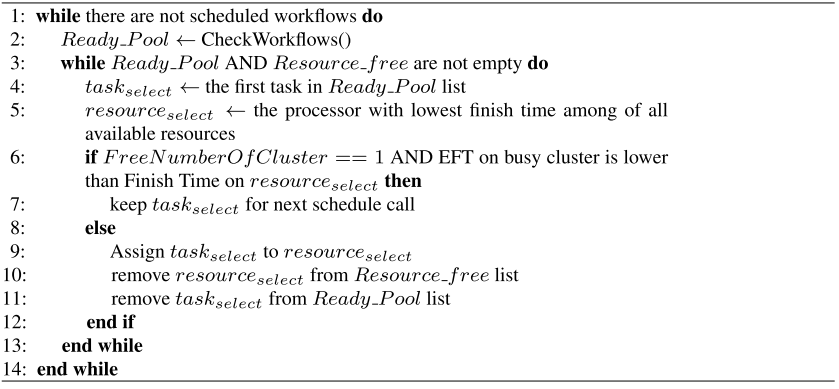
\includegraphics[width=0.6\textwidth]{owmAlg.png}
	\caption{Heurística do OWM}
	\label{ownAlg}
\end{figure}

A heurística do OW está formalizada na Figura \ref{ownAlg}.

\subsection{Algoritmo Fairness Dynamic Workflow Scheduling}
Arabnejad et al. \cite{Arabnejad2012} propuseram o algoritmo \textit{Fairness Dynamic Workflow Scheduling} (FDWS). O algoritmo FDWS implementa novas estratégia tanto no aspecto de seleção de tarefas da lista de tarefas disponíveis como na atribuiçao de processadores de modo a reduzir o \textit{Turnaround Time} individual dos \textit{workflows}. Este algoritmo tem 3 componentes principais. 
\begin{enumerate}
	\item \textit{Workflow Pool}
	\item Selecção de Tarefas
	\item Alocação de Processadores
\end{enumerate} 
A \textit{Workflow Pool} contém os \textit{workflows} submetido que chegam à medida que os utilizadores submetem os seus trabalhos. A cada ronda de escalonamento, este componente encontra todas as tarefas disponíveis de cada \textit{workflow}.
No algoritmo FDWS, tal como no algoritmo OWM, apenas uma tarefa disponível com a prioridade mais alta de cada DAG é adicionada à lista de tarefas prontas. Para atribuir a prioridade às tarefas, é utilizada a classificação $rank_u$ (Figura \ref{ranku}).

O componente de Seleção de Tarefas atribui uma classificação diferente para selecionar a tarefa a ser executada da lista de tarefas prontas. Para ser inserido na lista de tarefas prontas, a classificação $rank_u$ é calculada para cada \textit{workflow} individualmente. Para selecionar uma tarefa da lista, é calculado o $rank_r$ para cada tarefa $t_i$ pertencente a um DAG $DAG_j$, e a tarefa com maior classificação é selecionada. 

\begin{figure}[H]
	\centering
	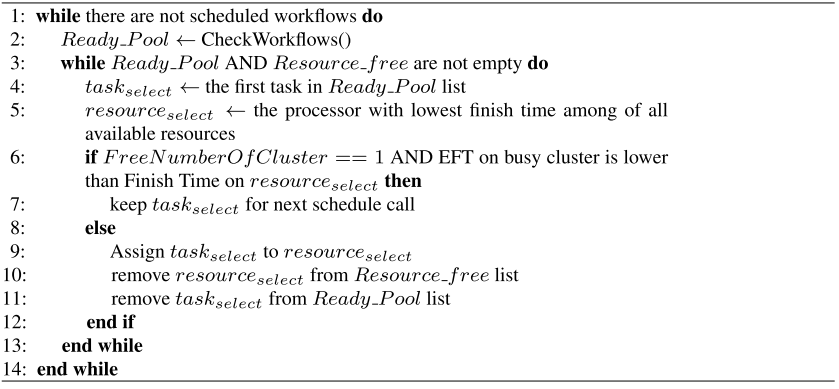
\includegraphics[width=0.6\textwidth]{owmAlg.png}
	\caption{Heurística do OWM}
	\label{Fórmula de $rank_u$}
\end{figure}

A fórmula do $rank_r$ pode ser vista na Figura \ref{rankr}. Esta métrica considera a percentagem de tarefas restantes (PRT, Percentage of Remaining Tasks) de um DAG e o seu comprimento do caminho crítico (CPL, Critical Path Length). O PRT dá mais prioridade a DAGs que estejam quase completos e tenham apenas um número de tarefas reduzido para executar. O CPL implemente uma estratégia diferente do que o tempo de processamento restante mais curto (SRPT, Smallest Remaining Processing Time) \cite{Maheswaran1999} que, a cada passo, seleciona e mapeia a aplicação com o menor tempo de processamento restante. O tempo restante de processamento é o tempo necessário para executar todas as tarefas restantes de um \textit{workflow}. No entanto, o tempo necessário para completar todas as tarefas de um DAG não tem em conta a largura de um DAG. Um DAG mais largo tem um CPL menor que outro DAG com o mesmo número de tarefas, tendo também um tempo esperado de conclusão mais baixo. Assim sendo, neste caso, o FDWS daria maior importância a DAGs com menores CPLs.

O componente de Alocação de Processadores apenas considera os processadores livres e o processador com o menor tempo de conclusão para a tarefa selecionada.

\begin{figure}[H]
	\centering
	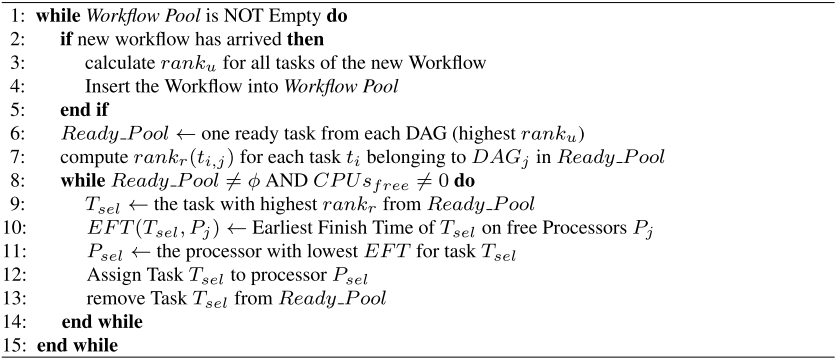
\includegraphics[width=0.6\textwidth]{fdwsAlg.png}
	\caption{Algoritmo FDWS}
	\label{fdwsAlg}
\end{figure}

Na Figura \ref{fdwsAlg} encontra-se a formalização do algoritmo FDWS.

\subsection{Algoritmo Multi-Workflow Deadline-Budget Scheduling}
O algoritmo Multi-Workflow Deadline-Budget Scheduling (MW-DBS), tem como objectivo encontrar uma solução de escalonamento de \textit{workflows} concorrentes tendo em conta restrições e orçamentos definidos pelos utilizadores. Este algoritmo é uma abordagem baseada em escalonamento de listas e, como tal, é composto por duas fases principais:
\begin{enumerate}
	\item Uma tarefa disponível de cada \textit{workflow} é selecionada e é-lhe atribuída uma prioridade baseada no seu \textit{deadline} (data e hora limite) individual.
	\item É determinado um recurso apropriado para executar a tarefa atual que satisfaz os parâmetros de QoS do \textit{workflow} a que a tarefa pertence.
\end{enumerate}
O algoritmo considera simultaneamente o orçamento do utilizador e as restrições de \textit{deadline} para executar o seu escalonamento \cite{ArabnejadUP}.

O MW-DBS foi concebido como uma estratégia heurística que em cada fase de seleção de processadores, obtém um mapeamento que cumpra sempre a restrição de custo (orçamento) e que possívelmente cumpra a restrição de \textit{deadline} do \textit{workflow} a que a tarefa pertence. Se a restrição de tempo for cumprida, é obtido um mapeamento bem-sucedido. Caso contrário  é considerado um falhanço e o \textit{workflow} deve ser terminado. O algoritmo é avaliado baseado na sua taxa de sucesso \cite{ArabnejadUP}.

Segue-se uma descrição mais detalhada das duas fases do algoritmo.

\subsubsection{Fase de seleção de tarefas}
Esta fase consiste na seleção da tarefa apropriada entre todas as tarefas disponíveis em cada \textit{workflow}. Geralmente, dois métodos são utilizados para preencher a lista de tarefas prontas.
\begin{enumerate}
	\item Obter uma única tarefa disponível de cada workflow \cite{Arabnejad2012}, \cite{Arabnejad2014}, \cite{Arabnejad2014a}, \cite{Hsu2011}.
	\item Obter todas as tarefas disponíveis pertencentes a cada \textit{workflow} por concluir \cite{Yu2008}.
\end{enumerate} 

Adicionar todas as tarefas disponíveis de cada workflow tem como resultado uma estratégia injusta, visto que o número elevado de tarefas disponíveis pode levar a que certos \textit{workflows} não participem na presente ronda de escalonamento. No algoritmo MW-DBS apenas uma tarefa, com o maior $rank_u$, é escolhida e adicionada à lista de tarefas prontas.
Assim sendo, é necessária uma segunda atribuição de prioridades baseadas nos parâmetros de QoS para atribuír uma classificação secundária a cada tarefa na list de tarefas prontas.
Como tanto o factor tempo como o de custo são restrições, a classificação secundária deve considerar ambas as medidas.
Para além disso, resultados em \cite{Arabnejad2012} e \cite{Arabnejad2014a} mostram que ter em conta o histórico do workflow das tarefas mapeadas leva a melhor performance.
Para este algoritmo foi utilizada uma nova classificação ($rank_D$) para atribuir uma prioridade secundária a cada tarefa $t_i$ pertencente a um workflow $j$ na lista de tarefas prontas. 

\begin{figure}[H]
	\centering
	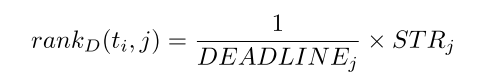
\includegraphics[width=0.6\textwidth]{rankD.png}
	\caption{Fórmula de $rank_D$}
	\label{rankD}
\end{figure}

A figura \ref{rankD} demonstra a fórmula do algoritmo $rank_D$, onde $DEADLINE_j$ é o \textit{deadline} de um \textit{workflow} $j$, o rácio de tarefas mapeadas (STR, Sheduled Tasks Ratio) $STR_j$ é o rácio entre número de tarefas mapeadas e o total de tarefas de um \textit{workflow} $j$.

O valor do $rank_D$ é o produto de dois factores:
\begin{enumerate}
	\item O inverso do factor de limitação de tempo \textit{deadline} para o workflow $j$, dando mais prioridade a \textit{workflows} submetidos e ainda não concluídos com menor valor de deadline.
	\item A fracção do \textit{workflow} j que está mapeado no sistema.
\end{enumerate}
A razão do primeiro factor é que o escalonador vai considerar primeiro \textit{workflows} que tenham menores limitações de tempo antes de falharem. A razão para o rácio de tarefas mapeadas é dar maior prioridade a \textit{workflows} que foram submetidos mais cedo, de forma a que um \textit{workflow} maior com várias tarefas já executadas possa ter prioridade sobre um \textit{workflow} pequeno mais recente.
No caso de dois \textit{workflows} terem a mesma \textit{deadline}, a tarefa que pertence ao \textit{workflow} com maior rácio de tarefas executadas terá prioridade.
Finalmente, a tarefa com o maior $rank_D$ na lista de tarefas prontas é selecionada para ser mapeada na fase seguinte.

\subsubsection{Fase de seleção de Processador}
Esta fase consiste na procura de um recurso apropriado para executar a tarefa selecionada.
Em ambas as fases, o algoritmo precisa de considerar os parâmetros de QoS de modo a ter soluções de maior qualidade e maior desempenho do sistema.
A fase de seleção de processador tem como objetivo selecionar um recurso acessível (em termos de custo) para a tarefa atual. Aqui foi proposta uma nova estratégia de seleção de processador baseada em parâmetros de QoS. Como cada workflow tem restrições de tempo e custo, ambos os parâmetros devem ser considerados na fase de seleção de processador. De modo a controlar o custo e tempo consumidos, um valor delimitado para cada fator é necessário.
Abaixo são descritos os primeiros valores delimitados para custo e tempo e de seguida a estratégia de seleção do processador.

\textbf{Limite de custo:} existe uma limitação no consumo do orçamento por parte da tarefa atual $t_curr$ baseada no orçamento utilizado por tarefas já executadas. No que toca a esta dissertação, o custo assumido vai ser sempre 1, visto que não é importante para os parâmetros de QoS estabelecidos.

\textbf{Limite de tempo:} Uma \textit{sub-deadline} baseada no \textit{deadline} do \textit{workflow} é atribuída a cada tarefa do workflow. É aplicada a estratégia de distribuição para planeamento de \textit{sub-deadlines} comum e direta.
O valor da \textit{sub-deadline} (DL) para cada tarefa $t_i$ é calculado recursivamente percorrendo o grafo de tarefas para cima, começando pera tarefa de saída. Neste caso, a \textit{sub-deadline} é definida considerando o tempo mínimo de execução da tarefa atual.

\begin{figure}[H]
	\centering
	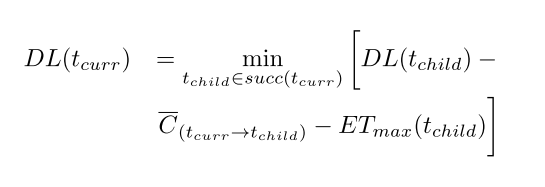
\includegraphics[width=0.6\textwidth]{mwdbsF1.png}
	\caption{Fórmula de cálculo da \textit{sub-deadline}}
	\label{mwdbsF1}
\end{figure}

\begin{figure}[H]
	\centering
	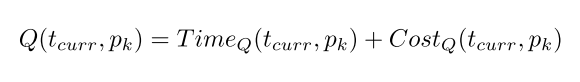
\includegraphics[width=0.6\textwidth]{mwdbsQ.png}
	\caption{Fórmula de cálculo da medida de qualidade $Q$}
	\label{mwdbsQ}
\end{figure}

\begin{figure}[H]
	\centering
	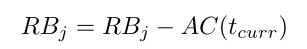
\includegraphics[width=0.3\textwidth]{mwdbsRB.png}
	\caption{Fórmula de cálculo do RB $Q$}
	\label{mwdbsRB}
\end{figure}

\begin{figure}[H]
	\centering
	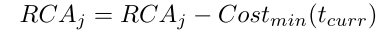
\includegraphics[width=0.38\textwidth]{mwdbsRCA.png}
	\caption{Fórmula de cálculo do RCA $Q$}
	\label{mwdbsRCA}
\end{figure}

Na figura \ref{mwdbsF1} podemos ver a fórmula para o cálculo da \textit{sub-deadline}, onde $ET_max$ simboliza o tempo máximo de execução da tarefa $t_curr$ entre os processadores disponíveis. Para a tarefa de saída, a \textit{sub-deadline} é igual à \textit{deadline} determinada pelo utilizador.

\begin{figure}[H]
	\centering
	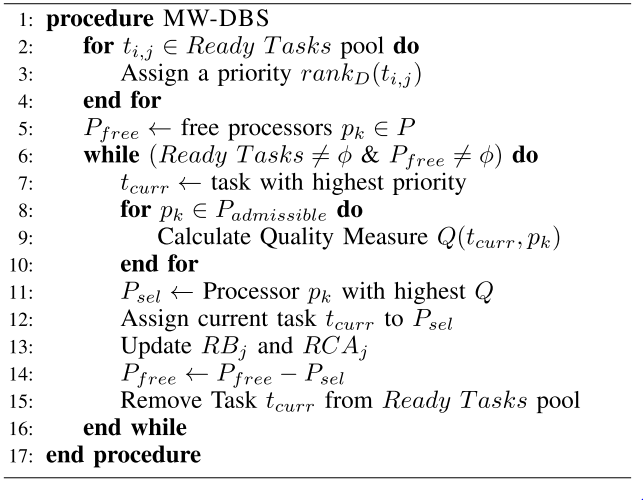
\includegraphics[width=0.6\textwidth]{mwdbsAlg.png}
	\caption{Algoritmo MW-DBS}
	\label{mwdbsAlg}
\end{figure}

O algoritmo MW-DBS pode ser visto na Figura \ref{mwdbsAlg}

O algoritmo funciona da seguinte forma:
\begin{itemize}
	\item todas as tarefas prontas na lista de tarefas prontas são classificadas pelo valor de prioridade $rank_D$.
	\item Para preencher a lista de tarefas prontas, o sistema recolhe uma única tarefa disponível com o maior valor de classificação primário $rank_u$ de cada \textit{workflow} submetido por executar.
	\item Enquanto houver pelo menos uma tarefa pronta e por mapear na lista de tarefas prontas e houverem processadores disponíveis, a tarefa pronta a executar atual $t_curr$ é selecionada e a sua medida de qualidade $Q$ (Figura \ref{mwdbsQ}) para todos os processadores admissíveis.
	\item A tarefa atual $t_curr$ é mapeada ao processador $P_sel$ que tem a maior medida de qualidade $Q$. 
	\item Finalmente, o orçamento não consumido restante (RB, Remaining Budget) (Figura \ref{mwdbsRB}) e a atribuição restante mais barata (RCA, Remain Cheapest Assignment) (Figura \ref{mwdbsRCA}) são atualizados para o workflow $j$ ao qual pertence a tarefa $t_curr$.
\end{itemize}

\subsection{Comparativo}
Nesta secção vão ser apresentadas algumas comparações entre os algoritmos acima mencionados.
Entre as principais diferenças entre os algoritmos, as principais são as seguintes:
\begin{enumerate}
	\item Enquanto que os algoritmos \textit{Rank Hybd} e \textit{OWM} dão mais importância à melhoria do tempo médio de finalização de todos os \textit{workflows}, o algoritmo FDWS privilegia na QoS experienciada por cada utilizador, minimizando os tempos de espera e execução de cada \textit{workflow} individual.
	\item O algoritmo MQMW é o único que considera o custo (monetário) da execução de um \textit{workflow}, o que é aplicável em situações em que o utilizador paga por ciclos de CPU, como por exemplo, alugando uma máquina num serviço \textit{Cloud} como o Microsoft Azure.
	\item Nos resultados apresentados em \cite{Hsu2011}, o algoritmo OWM obtém melhor performance que o Rank Hybd e o FDWS em \textit{workflows} on-line. 
	\item Tal como o algoritmo Rank Hybd, o algoritmo OWM usa uma estratégia justa, mas ao invés de mapear DAGs mais pequenos primeiro, seleciona e mapeia tarefas dos DAGs maiores primeiro. No entanto, o algoritmo OWM tem uma melhor estratégia para preencher a lista de taregas prontas, selecionando uma tarefa de cada DAG, para dar uma hipótese a todos os DAGs de serem escolhidos na mesma altura para mapeamento.
	\item Enquanto que o Rank Hybd adiciona todas as tarefas disponíveis à lista de tarefas prontas, o algoritmo OWM apenas adiciona uma tarefa disponível de cada DAG. Considerando todas as tarefas disponíveis de cada DAG leva a uma preferência imparcial para DAGs maiores e o consequente adiamento de DAGs mais pequenos, do qual resulta uma partilha do poder de processamento injusta. 
	\item Enquanto que os algoritmos Rank Hybd e OWM usam apenas o $rank_u$ para selecionar tarefas a adicionar à lista de tarefas prontas, tanto o FDWS como o MW-DBS utilizam métricas de classificação secundárias que tomam em conta o historial de um DAG na lista de tarefas prontas.
\end{enumerate}
	
\section{SIMGRID}
Nesta dissertação vai ser utilizada uma simulação para avaliar os algoritmos da secção \ref{sec:schalg}.
Os simuladores permitem executar um número de testes estatisticamente significante numa configuração de máquinas definida pelo utilizador. Nesta dissertação, é utilizado o \textit{toolkit} SIMGRID \cite{Casanova2008} como base para as nossas simulações.
O SIMGRID disponibiliza as abstrações fundamentais necessárias à simulação de eventos discretos de aplicações paralelas em ambientes distribuídos. Foi especialmente desenvolvido para a avaliação de algoritmos de escalonamento.
Basear-nos num \textit{toolkit} de simulação bem estabelecido permite-nos tirar vantagem de modelos robustos de sistemas distribuídos.
Em muitos artigos de pesquisa sobre escalonamento, os autores assumem um modelo de rede em que os processadores podem simultaneamente enviar ou receber dados de tantos processadores como determinarem, isto sem que sejam prejudicados em termos de performance. Este tipo de modelo, denominado \textit{multi-port} não reflete uma rede numa infraestrutura. Inversamente, o modelo de rede disponibilizado pelo SIMGRID corresponde a um modelo \textit{multi-port} teoreticamente delimitado. Neste modelo, um processador pode comunicar com vários outros simultaneamente, mas cada fluxo de comunicação é limitado pela largura de banda da rota percorrida, e comunicações que usam uma ligação comum têm que partilhar a largura de banda disponível. Isto corresponde ao comportamento de ligações TCP numa rede LAN. A validade deste modelo de rede foi demonstrado em \cite{Velho2009}.



